%% Random Walks: From Mathematical Foundations to Modern AI
%% IEEE Conference template (IEEEtran.cls)
%% Compile on Overleaf or with a local TeX Live distribution that includes
%% the texlive-publishers package.

\documentclass[conference,a4paper,10pt]{IEEEtran}
\IEEEoverridecommandlockouts

\usepackage{cite}
\usepackage{amsmath,amssymb,amsfonts}
\usepackage{amsthm}
\usepackage{algorithmic}
\usepackage{graphicx}
\usepackage{textcomp}
\usepackage{xcolor}
\usepackage{booktabs}
\usepackage{url}
\usepackage[hidelinks]{hyperref}

\newtheorem{theorem}{Theorem}
\newtheorem{definition}{Definition}

\def\BibTeX{{\rm B\kern-.05em{\sc i\kern-.025em b}\kern-.08em
    T\kern-.1667em\lower.7ex\hbox{E}\kern-.125emX}}

\begin{document}

\title{Random Walks: From Mathematical Foundations\\
to Modern Applications in Artificial Intelligence}

\author{
\IEEEauthorblockN{Kam Seng Lei}
\IEEEauthorblockA{The Hong Kong University of Science\\
and Technology (Guangzhou)\\
Guangzhou, Guangdong, China}
\and
\IEEEauthorblockN{Kaige Liang}
\IEEEauthorblockA{The Hong Kong University of Science\\
and Technology (Guangzhou)\\
Guangzhou, Guangdong, China}
}

\maketitle

\begin{abstract}
The random walk is one of the most influential mathematical objects in
probability theory and a foundational primitive throughout modern artificial
intelligence (AI). In this report we trace the concept from its simplest
incarnation~--- a one-dimensional walk driven by independent coin flips~---
to its quantitative consequences (linear drift, $\sqrt{n}$ diffusion, and
the central limit theorem) and to its dimensional behaviour as captured by
P\'{o}lya's recurrence theorem. We then survey how the random-walk
abstraction is used inside contemporary AI: it underpins Google's PageRank,
the noising/denoising mechanism of diffusion-based generative models,
random-walk graph embeddings such as DeepWalk and node2vec, Markov chain
Monte Carlo (MCMC) inference, and exploration in reinforcement learning.
The report also documents how we prepared the class demonstration: each
formula is paired with a visual simulation or AI example so that the
concept is both mathematically precise and easy to explain. The
accompanying GitHub Pages supplement is available at
\url{https://kaigeliang.github.io/random-walks-ai-report/}.
\end{abstract}

\begin{IEEEkeywords}
random walk, central limit theorem, Markov chain, P\'{o}lya's theorem,
PageRank, diffusion model, graph embedding, MCMC, reinforcement learning
\end{IEEEkeywords}

%% =============================================================
\section{Introduction}
%% =============================================================
Stock prices, the trajectory of a pollen grain in water, the path of a web
surfer clicking from page to page, the noise schedule of a modern image
generator~--- on the surface, these phenomena have very little in common.
What unites them is a deceptively simple mathematical object: the
\emph{random walk}.

A random walk is a path built from a sequence of random steps. At every
moment, ``chance'' decides where the walker goes next, independently of
where it has been. Repeat that rule many times, and the walker traces out a
jagged, erratic trajectory whose statistical regularities are remarkably
deep~\cite{spitzer2001random,lawler2010random}. The randomness at the level
of a single step gives rise to surprisingly rigid order at the level of the
ensemble: a linear average drift, a spread that grows like the square root
of time, and~--- in the limit~--- the universal bell curve of the central
limit theorem (CLT).

Historically the random walk has a remarkable lineage. The term was
coined by Karl Pearson in a 1905 letter to \emph{Nature} in which he asked
how far a drunk man would have wandered after $n$ steps. Five years
earlier, Louis Bachelier had used essentially the same model to study
fluctuations on the Paris stock exchange in his Sorbonne thesis, and in
1905 Albert Einstein independently invoked it to predict the motion of
particles suspended in a fluid~--- a result that Jean Perrin later turned
into experimental evidence for the existence of atoms. The same object
underpinned Andrey Markov's analysis of letter dependencies in
\emph{Eugene Onegin}, and reappeared in George P\'{o}lya's celebrated 1921
recurrence theorem. A century on, it remains a load-bearing primitive in
machine learning, network science, and statistical physics.

This report has three goals. First, in Section~\ref{sec:prep} we document
how we prepared the demonstration and then lay out the probabilistic
background needed to make the walk precise. Second, in
Sections~\ref{sec:1d} and~\ref{sec:dim} we develop the mathematics of the
one-dimensional walk and its higher-dimensional extensions, recovering the
results presented in our class talk. Third, and most importantly,
Section~\ref{sec:ai} explains how the random-walk abstraction is reused
across modern AI: ranking, generation, embedding, inference, and
exploration. Section~\ref{sec:conclusion} concludes.

%% =============================================================
\section{Preparation}\label{sec:prep}
%% =============================================================
Our project was prepared as a two-layer demonstration. The first layer
builds intuition from one fair coin walk: we show individual sample paths,
the $\sqrt{n}$ envelope, the CLT histogram, and the recurrence contrast in
low versus high dimensions. The second layer reuses the same transition
rule inside AI systems, so the audience can see that PageRank, diffusion
models, graph embeddings, MCMC, and RL exploration are not isolated
examples but different algorithmic uses of the same random-walk idea.
Kam Seng Lei led the mathematical storyline, including the definitions,
drift and variance derivations, CLT explanation, P\'{o}lya theorem
summary, and reference checking. Kaige Liang led the computational and AI
storyline, including the Python simulations, figures, PageRank and
diffusion examples, and the mapping from each equation to a machine
learning application. Both members rehearsed the demonstration together,
cross-checked equations and captions, and edited the final report for
clarity and consistency.

To make the static report easier to present and reproduce, we also built
a lightweight interactive supplement for GitHub Pages. The page is stored
in \texttt{docs/index.html} in the project repository and animates the
same five AI examples discussed in Section~\ref{sec:ai}: the PageRank
random surfer, forward diffusion noising, DeepWalk-style graph sampling,
random-walk Metropolis inference, and $\epsilon$-greedy exploration in
reinforcement learning. This supplement is not a separate model or
experimental claim; it is a visual companion to the equations and figures
used in the report. The live version is available at
\url{https://kaigeliang.github.io/random-walks-ai-report/}.

We model uncertainty on a probability space $(\Omega,\mathcal{F},\mathbb{P})$
in the standard Kolmogorov sense~\cite{durrett2019probability}. A
real-valued \emph{random variable} $X:\Omega\to\mathbb{R}$ has expectation
$\mathbb{E}[X]=\int X\,d\mathbb{P}$ and variance
$\mathrm{Var}(X)=\mathbb{E}[(X-\mathbb{E}[X])^{2}]$. Two key properties drive
everything that follows.

\begin{enumerate}
\item \textbf{Linearity of expectation.} For any random variables
$X_{1},\dots,X_{n}$ and constants $a_{i}$,
\begin{equation}
\mathbb{E}\!\left[\sum_{i=1}^{n}a_{i}X_{i}\right]
=\sum_{i=1}^{n}a_{i}\,\mathbb{E}[X_{i}],
\label{eq:linexp}
\end{equation}
regardless of whether the $X_{i}$ are independent.
\item \textbf{Variance of independent sums.} If $X_{1},\dots,X_{n}$ are
\emph{independent}, then
\begin{equation}
\mathrm{Var}\!\left(\sum_{i=1}^{n}X_{i}\right)
=\sum_{i=1}^{n}\mathrm{Var}(X_{i}).
\label{eq:varsum}
\end{equation}
Independence is essential here: cross-terms vanish only because the
covariances are zero.
\end{enumerate}

A sequence $X_{1},X_{2},\dots$ that is \emph{independent and identically
distributed}~(i.i.d.) is the basic building block of a random walk: every
step is drawn from the same distribution, and no step has any memory of
the previous ones. The discrete-time stochastic process
$\{S_{n}\}_{n\geq 0}$ obtained by partial summation of i.i.d.\ steps is
itself a Markov chain on the integers (or on $\mathbb{Z}^{d}$, or on a
graph), since the next state depends on the past only through the present.
This \emph{Markov property} is the hinge that connects elementary random
walks to the broader theory of stochastic processes:
\begin{multline}
\mathbb{P}\bigl(S_{n+1}=y\mid S_{n}=x,\,S_{n-1},\dots,S_{0}\bigr)\\
=\mathbb{P}\bigl(S_{n+1}=y\mid S_{n}=x\bigr).
\end{multline}
Many of the AI applications surveyed in Section~\ref{sec:ai} ultimately
reduce to algorithmic exploitation of this single equation.

%% =============================================================
\section{The One-Dimensional Random Walk}\label{sec:1d}
%% =============================================================

\subsection{Setup}
Place a walker at the origin. At every discrete time step the walker takes
a step of size one to the right or to the left, with probabilities
$p$ and $1-p$ respectively. Formally, let
\begin{equation}
X_{i}=
\begin{cases}
+1 & \text{with probability } p, \\
-1 & \text{with probability } 1-p,
\end{cases}
\label{eq:step}
\end{equation}
i.i.d.\ across $i$. The position after $n$ steps is the random variable
\begin{equation}
S_{n}=\sum_{i=1}^{n}X_{i},\qquad S_{0}=0.
\label{eq:Sn}
\end{equation}

\subsection{Average behaviour: linear drift}
Equation~\eqref{eq:step} gives
\begin{equation}
\mathbb{E}[X_{i}]=p\cdot(+1)+(1-p)\cdot(-1)=2p-1.
\label{eq:Estep}
\end{equation}
By linearity~\eqref{eq:linexp},
\begin{equation}
\mathbb{E}[S_{n}]=n(2p-1).
\label{eq:ESn}
\end{equation}
For a fair coin ($p=\tfrac{1}{2}$) the walk is unbiased: $\mathbb{E}[S_{n}]
=0$ for all $n$. A small bias produces a sizeable drift over many steps:
$p=0.51$ and $n=10{,}000$ already give $\mathbb{E}[S_{n}]=200$.

\subsection{Spread: the \texorpdfstring{$\sqrt{n}$}{sqrt(n)} envelope}
The single-step variance is
\begin{equation}
\mathrm{Var}(X_{i})
=\mathbb{E}[X_{i}^{2}]-\mathbb{E}[X_{i}]^{2}
=1-(2p-1)^{2}=4p(1-p).
\end{equation}
Because the steps are independent, \eqref{eq:varsum} immediately gives
\begin{equation}
\mathrm{Var}(S_{n})=n\bigl[1-(2p-1)^{2}\bigr]=4np(1-p),
\label{eq:VarSn}
\end{equation}
so the standard deviation scales like $\sqrt{n}$. For a fair coin
$\mathrm{Var}(S_{n})=n$ and $\sigma(S_{n})=\sqrt{n}$.

\begin{figure}[!htbp]
\centering
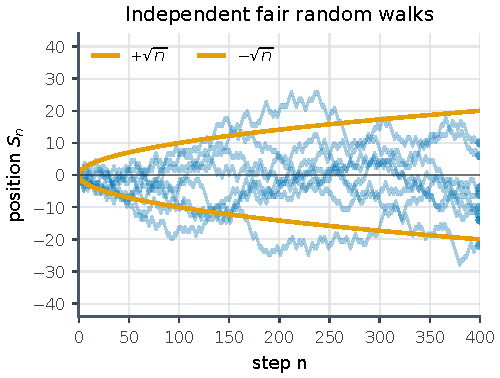
\includegraphics[width=0.97\columnwidth]{fig_walks.pdf}
\caption{Eight independent fair walks of length $400$. The deterministic
$\pm\sqrt{n}$ envelope (gold) tracks the typical magnitude of $S_{n}$:
the cloud widens, but only sub-linearly.}
\label{fig:walks}
\end{figure}

The qualitative consequence is striking: ten times more steps only widens
the typical distance from the origin by a factor of
$\sqrt{10}\approx 3.16$. After $100$ fair steps the walker is typically
about $10$ units from the start, not $50$. Figure~\ref{fig:walks} shows
eight independent walks together with the $\pm\sqrt{n}$ envelope.

\subsection{Central limit theorem}
The most striking regularity emerges when we rescale. Define
\begin{equation}
Z_{n}=\frac{S_{n}-n(2p-1)}{\sqrt{n\bigl[1-(2p-1)^{2}\bigr]}}.
\end{equation}
The classical Lindeberg--L\'{e}vy CLT~\cite{durrett2019probability} states
that $Z_{n}\xrightarrow{d}\mathcal{N}(0,1)$ as $n\to\infty$, where the
arrow denotes convergence in distribution. For the symmetric coin walk
this simplifies to
\begin{equation}
\frac{S_{n}}{\sqrt{n}}\xrightarrow{d}\mathcal{N}(0,1).
\label{eq:CLT}
\end{equation}
Empirically, the histogram of the rescaled walk converges to the standard
Gaussian as $n$ grows; see Fig.~\ref{fig:clt}. This is the universality
result: regardless of the fine details of the step distribution (as long
as it has finite variance), the macroscopic shape of the walk is a bell
curve.

\begin{figure*}[!t]
\centering
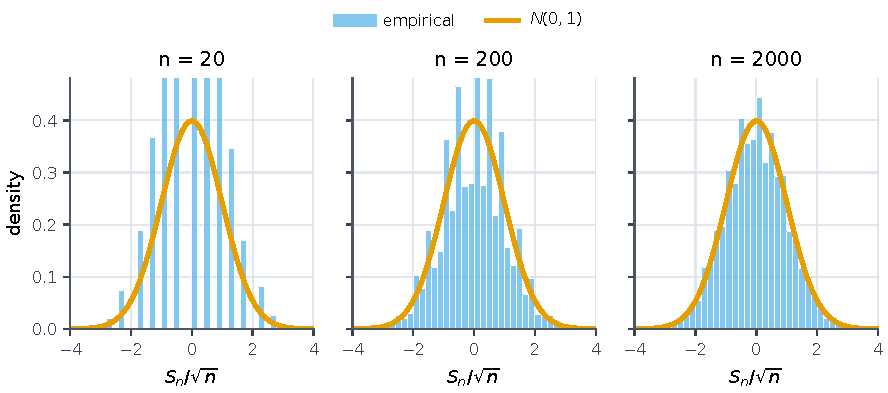
\includegraphics[width=0.95\textwidth]{fig_clt.pdf}
\caption{Empirical density of $S_{n}/\sqrt{n}$ for a fair walk with
$N=12{,}000$ replicates and $n\in\{20,200,2000\}$. The gold curve is the
standard normal $\mathcal{N}(0,1)$. Larger $n$ produces a closer match
between the histogram and the limiting Gaussian.}
\label{fig:clt}
\end{figure*}

\subsection{Diffusive scaling and Brownian motion}
The $\sqrt{n}$ growth and the Gaussian limit are two faces of the same
phenomenon: the random walk is a discrete approximation of \emph{Brownian
motion}~\cite{morters2010brownian}. If we shrink the spatial step to $\Delta
x=\sqrt{\Delta t}$ and the time step to $\Delta t\to 0$, the rescaled walk
converges (in the sense of Donsker's invariance principle) to standard
Brownian motion $B_{t}$, a continuous-time process with independent,
Gaussian increments. The same diffusive scaling will reappear later in
this report when we discuss generative diffusion models.

%% =============================================================
\section{Higher Dimensions and P\'{o}lya's Theorem}\label{sec:dim}
%% =============================================================
The simple random walk generalises naturally to the integer lattice
$\mathbb{Z}^{d}$. At each step the walker chooses one of the $2d$ axial
neighbours uniformly at random. The expectation and variance arguments
of Section~\ref{sec:1d} carry over coordinate-wise; the
$\sqrt{n}$ scaling is unchanged.

What changes dramatically with dimension is the question of
\emph{recurrence}.

\begin{definition}
A random walk is \emph{recurrent} if it returns to its starting point
with probability one, and \emph{transient} otherwise.
\end{definition}

\begin{theorem}[P\'{o}lya, 1921~\cite{polya1921}]
The simple symmetric random walk on $\mathbb{Z}^{d}$ is recurrent for
$d\in\{1,2\}$ and transient for $d\geq 3$.
\end{theorem}

The contrast is famously summarised by Kakutani's quip: \emph{a drunk
man will eventually find his way home, but a drunk bird may get lost
forever}. The proof inspects the expected number of returns to the origin,
\begin{equation}
\mathbb{E}\!\left[\sum_{n=0}^{\infty}\mathbf{1}\{S_{n}=0\}\right]
=\sum_{n=0}^{\infty}\mathbb{P}(S_{n}=0),
\end{equation}
and uses the local CLT to show $\mathbb{P}(S_{n}=0)\sim C n^{-d/2}$. The
series diverges for $d\le 2$ (forcing recurrence) and converges for
$d\ge 3$ (allowing escape).

This dimensional dichotomy is far from a curiosity. It says something
deep about the geometry of randomness: in low dimensions there is
``not enough room'' to escape, so paths self-intersect repeatedly, while
in high dimensions there is ``too much room'', and a typical path
escapes to infinity. Both regimes are exploited in modern AI~--- often,
remarkably, in the same algorithm.

%% =============================================================
\section{Applications in Artificial Intelligence}\label{sec:ai}
%% =============================================================

The random walk is not merely a mathematical curiosity~--- it is a working
primitive inside several pillars of modern AI. We organise the discussion
around five representative applications.

\subsection{PageRank and link-based ranking}
Google's original ranking algorithm, PageRank~\cite{page1999pagerank},
models a hypothetical \emph{random surfer}: a user that, at each step,
either clicks a uniformly chosen link on the current page (with
probability $1-\alpha$) or teleports to a uniformly chosen page (with
probability $\alpha\approx 0.15$). This defines an irreducible, aperiodic
Markov chain on the web graph. The PageRank score of a page is the
stationary probability that the surfer occupies that page in the
long run.

\begin{figure}[!htbp]
\centering
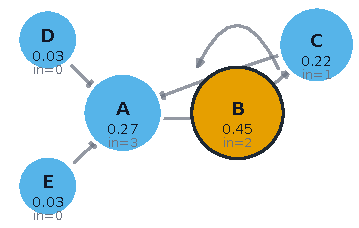
\includegraphics[width=0.85\columnwidth]{fig_pagerank.pdf}
\caption{Toy web graph with five pages. The stationary distribution of
the random-surfer Markov chain assigns the highest probability mass to
the most ``trafficked'' node (gold), regardless of its raw in-degree.}
\label{fig:pagerank}
\end{figure}

Figure~\ref{fig:pagerank} illustrates the idea on a five-page toy graph:
the gold node is the one a random surfer occupies most often in the long
run, even though it does not have the highest raw in-degree.
Concretely, if $A$ is the column-stochastic transition matrix and
$\mathbf{e}$ the uniform vector, the PageRank vector $\mathbf{r}$
satisfies
\begin{equation}
\mathbf{r}=(1-\alpha)A\mathbf{r}+\alpha\mathbf{e},
\end{equation}
which is solved efficiently by power iteration. The teleportation term
guarantees recurrence~--- exactly the property P\'{o}lya's theorem
formalises~--- and therefore a unique stationary distribution.
Link-prediction systems, citation analysis, recommendation engines, and
fraud-detection pipelines all extend or specialise this random-walk
formulation~\cite{gleich2015pagerank}. \emph{Personalised} PageRank,
which biases the teleportation distribution toward a query node, is
particularly popular in recommender systems: it captures the intuition
that pages frequently visited from a seed are likely relevant to a user
who has just viewed that seed.

\subsection{Diffusion models for generative AI}
Modern image, audio, and video generators (Stable Diffusion, Imagen, Sora,
\dots) are built around \emph{denoising diffusion probabilistic models}
(DDPMs)~\cite{ho2020ddpm}. Their forward process is, quite literally, a
random walk in pixel space: starting from a clean datum $x_{0}$, one adds
small Gaussian increments,
\begin{equation}
x_{t}=\sqrt{1-\beta_{t}}\,x_{t-1}+\sqrt{\beta_{t}}\,\epsilon_{t},
\quad \epsilon_{t}\sim\mathcal{N}(0,I),
\end{equation}
until $x_{T}$ is indistinguishable from pure noise. The continuous-time
limit is exactly the Brownian motion described in
Section~\ref{sec:1d}~\cite{song2021scorebased}.
Figure~\ref{fig:diffusion} traces a one-dimensional toy example: a
clearly bimodal data distribution at $t=0$ is gradually smeared by
Gaussian increments until, at $t=T$, it is statistically
indistinguishable from $\mathcal{N}(0,1)$. Generation is the time
\emph{reverse} of this walk: a neural network is trained to estimate the
score $\nabla_{x}\log p_{t}(x)$ at every noise level, and a numerical SDE
solver runs the diffusion backwards from $x_{T}$ to $x_{0}$. The
$\sqrt{n}$ spreading we proved in Eq.~\eqref{eq:VarSn} is the very reason
the noising schedule must be square-root in time; the CLT
\eqref{eq:CLT} is the reason the limiting distribution is tractable
Gaussian.

\begin{figure}[!htbp]
\centering
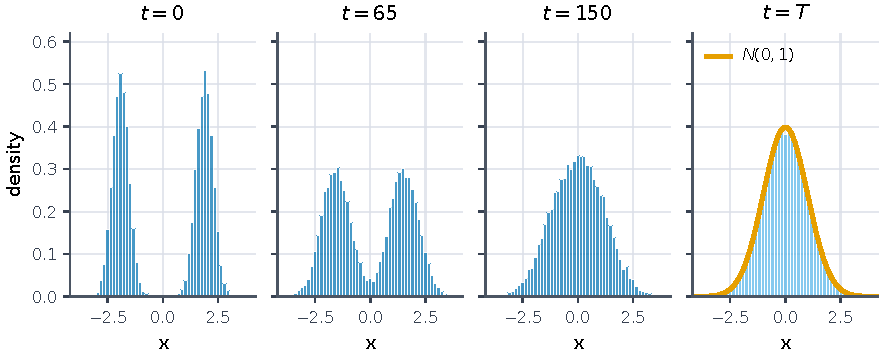
\includegraphics[width=0.98\columnwidth]{fig_diffusion.pdf}
\caption{Forward diffusion on a one-dimensional toy distribution. A
clean bimodal $x_{0}$ (left) is gradually noised by a Gaussian random
walk until $x_{T}$ matches the standard normal (gold reference).
Generation reverses this walk via a learned score model.}
\label{fig:diffusion}
\end{figure}

\subsection{Random-walk graph embeddings: DeepWalk and node2vec}
Representing graph nodes as low-dimensional vectors is a central problem
in network analysis. DeepWalk~\cite{perozzi2014deepwalk} treats short
random walks on a graph as ``sentences'' and feeds them to a Skip-gram
language model: nodes that co-occur on the same walk receive similar
embeddings (Fig.~\ref{fig:deepwalk}).

\begin{figure}[!htbp]
\centering
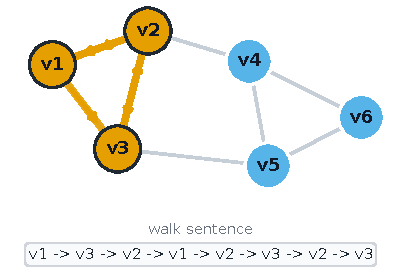
\includegraphics[width=0.95\columnwidth]{fig_deepwalk.pdf}
\caption{A short random walk on a graph (gold path) plays the role of a
``sentence'' in DeepWalk and node2vec. The Skip-gram objective then
pulls the embeddings of co-occurring nodes together, producing
neighbourhood-aware vector representations.}
\label{fig:deepwalk}
\end{figure}

The node2vec method~\cite{grover2016node2vec} generalises this with a
biased walk that interpolates between breadth-first (homophily) and
depth-first (structural equivalence) exploration:
\begin{equation}
\pi(v\to x \mid t)=
\begin{cases}
1/p & d_{tx}=0, \\
1   & d_{tx}=1, \\
1/q & d_{tx}=2,
\end{cases}
\end{equation}
where $d_{tx}$ is the shortest-path distance from the previous node $t$
to the candidate $x$. These embeddings have been used to predict drug
interactions, recommend products on Pinterest, classify proteins, and
detect financial fraud~--- always exploiting the random walk as a
neighbourhood sampler. Personalised PageRank, computed from short random
walks rooted at a query node, plays the same role inside more recent
graph neural networks~\cite{klicpera2019appnp}.

\subsection{Markov chain Monte Carlo}
Whenever a probability distribution $\pi(x)$ is known only up to a
constant~--- as is typical for Bayesian posteriors and energy-based
models~--- it can still be sampled by constructing a Markov chain whose
stationary distribution is $\pi$. The Metropolis--Hastings random walk
proposes $x'\sim q(x'\mid x_{t})$, accepts with probability
\begin{equation}
\alpha(x_{t},x')=\min\!\left\{1,\,\frac{\pi(x')\,q(x_{t}\mid x')}
{\pi(x_{t})\,q(x'\mid x_{t})}\right\},
\end{equation}
and otherwise stays put~\cite{hastings1970}. Hamiltonian Monte Carlo
(HMC) and Langevin dynamics use Brownian-motion proposals derived from
the gradient of $\log\pi$. Figure~\ref{fig:mcmc} shows a small
Metropolis chain exploring a banana-shaped target: a few dozen steps
trace the random walker's path through the support, and after a few
thousand the empirical distribution of the chain matches the contours
of the target.

\begin{figure}[!htbp]
\centering
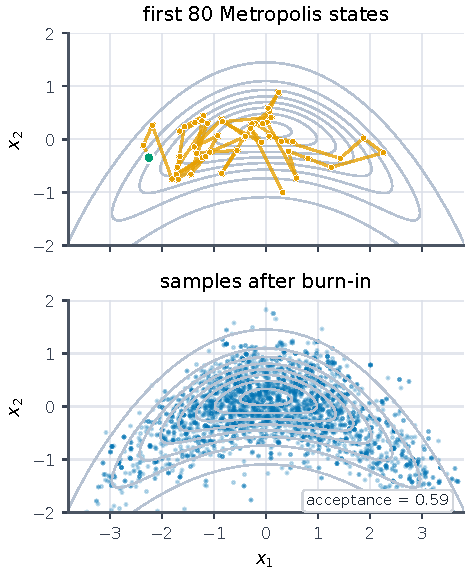
\includegraphics[width=0.85\columnwidth]{fig_mcmc.pdf}
\caption{Random-walk Metropolis on a two-dimensional banana-shaped
target. \textbf{Top:} the first $80$ samples (gold dots) traced by the
proposal--accept random walk, overlaid on the target's level sets.
\textbf{Bottom:} after $4000$ steps the empirical distribution of the
chain (navy dots) faithfully tracks the target. Mixing time controls
how fast this match is achieved.}
\label{fig:mcmc}
\end{figure}

MCMC underpins probabilistic programming
languages (Stan, PyMC), Bayesian deep learning, posterior inference in
modern diffusion samplers, and the training of restricted Boltzmann
machines. The convergence rate of these algorithms is exactly a
random-walk mixing-time question~\cite{levin2017markov}: poorly chosen
proposal kernels diffuse too slowly to escape a local mode, while
overly aggressive ones reject most moves. Tuning these random walks
~--- adaptive step sizes, parallel tempering, gradient-informed
proposals~--- is one of the most active areas in computational
statistics.

\subsection{Exploration in reinforcement learning}
Reinforcement-learning (RL) agents must \emph{explore} an unknown
environment before they can exploit it. A classical baseline is the
$\epsilon$-greedy policy that chooses a random action with probability
$\epsilon$~--- a random walk on the action space. More sophisticated
strategies still rely on the random-walk abstraction: option-critic
methods discover sub-policies via random walks on the state graph,
successor-feature methods compute occupancy measures that are exactly
the visit frequencies of a random walk, and ``go-explore'' style
algorithms~\cite{ecoffet2021goexplore} use random walks from previously
visited cells to discover novel states. The exploration-exploitation
trade-off can be expressed as a random walk with a learnt bias~--- the
RL analogue of choosing the parameter $p$ in
Eq.~\eqref{eq:step}.

\subsection{A unifying view}
Across these five families a common pattern emerges. The forward random
walk produces samples from a target stationary distribution (PageRank,
MCMC), or it noises a signal in a controlled way (diffusion models). The
walk's structural properties~--- linear drift, $\sqrt{n}$ spread, the
Gaussian limit of Eq.~\eqref{eq:CLT}, and the recurrence/transience
dichotomy of P\'{o}lya's theorem~--- determine whether the algorithm
mixes, converges, generalises, or escapes. Far from being an introductory
example in a probability course, the random walk is a load-bearing
abstraction inside the systems we use every day.

%% =============================================================
\section{Conclusion}\label{sec:conclusion}
%% =============================================================
We started from a coin: heads we step right, tails we step left. With
nothing more than the linearity of expectation and the additivity of
variance over independent summands, we derived the linear drift
$\mathbb{E}[S_{n}]=n(2p-1)$ and the diffusive spread
$\sigma(S_{n})=\sqrt{4np(1-p)}$. Taking the limit gave the central limit
theorem; lifting to higher dimensions exposed P\'{o}lya's recurrence
dichotomy. We then traced the same abstraction through five active
research areas in AI: PageRank, diffusion-based generative models, random-walk
graph embeddings, MCMC inference, and exploration in reinforcement
learning. The lesson of the report is that elementary probability,
properly understood, scales: the same coin flip we analysed in
Section~\ref{sec:1d} powers the algorithms behind today's most
sophisticated AI systems.

\clearpage
\bibliographystyle{IEEEtran}
\begin{thebibliography}{99}
\scriptsize
\setlength{\itemsep}{-1pt}
\setlength{\parsep}{0pt}
\setlength{\parskip}{0pt}

\bibitem{spitzer2001random}
F.~Spitzer, \emph{Principles of Random Walk}, 2nd~ed.\ \ New York, NY, USA:
Springer, 2001.

\bibitem{lawler2010random}
G.~F.~Lawler and V.~Limic, \emph{Random Walk: A Modern Introduction}.\ \
Cambridge, U.K.: Cambridge Univ.\ Press, 2010.

\bibitem{durrett2019probability}
R.~Durrett, \emph{Probability: Theory and Examples}, 5th~ed.\ \ Cambridge,
U.K.: Cambridge Univ.\ Press, 2019.

\bibitem{morters2010brownian}
P.~M\"{o}rters and Y.~Peres, \emph{Brownian Motion}.\ \ Cambridge, U.K.:
Cambridge Univ.\ Press, 2010.

\bibitem{polya1921}
G.~P\'{o}lya, ``\"{U}ber eine Aufgabe der Wahrscheinlichkeitsrechnung
betreffend die Irrfahrt im Stra\ss ennetz,'' \emph{Mathematische Annalen},
vol.~84, no.~1--2, pp.~149--160, 1921.

\bibitem{page1999pagerank}
L.~Page, S.~Brin, R.~Motwani, and T.~Winograd, ``The PageRank citation
ranking: Bringing order to the web,'' Stanford InfoLab, Tech.\ Rep.\
1999--66, 1999.

\bibitem{gleich2015pagerank}
D.~F.~Gleich, ``PageRank beyond the web,'' \emph{SIAM Review}, vol.~57,
no.~3, pp.~321--363, 2015.

\bibitem{ho2020ddpm}
J.~Ho, A.~Jain, and P.~Abbeel, ``Denoising diffusion probabilistic
models,'' in \emph{Proc.\ NeurIPS}, vol.~33, 2020, pp.~6840--6851.

\bibitem{song2021scorebased}
Y.~Song, J.~Sohl-Dickstein, D.~P.~Kingma, A.~Kumar, S.~Ermon, and B.~Poole,
``Score-based generative modeling through stochastic differential
equations,'' in \emph{Proc.\ ICLR}, 2021.

\bibitem{perozzi2014deepwalk}
B.~Perozzi, R.~Al-Rfou, and S.~Skiena, ``DeepWalk: Online learning of
social representations,'' in \emph{Proc.\ ACM SIGKDD}, 2014, pp.~701--710.

\bibitem{grover2016node2vec}
A.~Grover and J.~Leskovec, ``node2vec: Scalable feature learning for
networks,'' in \emph{Proc.\ ACM SIGKDD}, 2016, pp.~855--864.

\bibitem{klicpera2019appnp}
J.~Klicpera, A.~Bojchevski, and S.~G\"{u}nnemann, ``Predict then propagate:
Graph neural networks meet personalized PageRank,'' in \emph{Proc.\ ICLR},
2019.

\bibitem{hastings1970}
W.~K.~Hastings, ``Monte Carlo sampling methods using Markov chains and
their applications,'' \emph{Biometrika}, vol.~57, no.~1, pp.~97--109, 1970.

\bibitem{levin2017markov}
D.~A.~Levin and Y.~Peres, \emph{Markov Chains and Mixing Times}, 2nd~ed.\ \
Providence, RI, USA: AMS, 2017.

\bibitem{ecoffet2021goexplore}
A.~Ecoffet, J.~Huizinga, J.~Lehman, K.~O.~Stanley, and J.~Clune,
``First return, then explore,'' \emph{Nature}, vol.~590, no.~7847,
pp.~580--586, 2021.

\end{thebibliography}

\end{document}
